\section{Лекция номер 12}

\subsection{Многомерный Тейлор}
\begin{theorem} (Многомерная формула Тейлора)
    
    $D \subset \R^n$ -- открытое, $f \in C^{r+1}(D)$ и $[a, x] \subset D$.
    Тогда существует такое $\Theta \in (0, 1)$, что:
    \begin{gather*}
        f(x) = \sum\limits_{\abs{k} \leqslant r} \frac{f^{(k)}(a)}{k!}(x-a)^k + \sum\limits_{\abs{k} = r+1} \frac{f^{(k)}(a + \Theta(x-a))}{k!}(x-a)^k
    \end{gather*}
    \underline{Мини-замечание}: Все действия производятся с мультииндексами
\end{theorem}
\begin{proof}
    Доказательство не слишком мудрёное, в основном мы пользуемся леммой, которую мы только-только доказали. 
    Введем $F(t) := f(a + th)$ и $h = x - a$. Напишем адекватного Тейлора для $F$ в единице, с остатком в форме Лагранжа: 
    \begin{gather*}
        F(1) = \sum\limits_{j=0}^r \frac{F^{(j)}(0)}{j!} + \frac{F^{(r+1)}(\Theta)}{(r+1)!} 
    \end{gather*}
    Теперь воспользуемся леммой, чтобы разложить производные $F$ разных порядков и выразим $f(x)$:
    \begin{gather*}
        f(x) = F(1) = \sum\limits_{j=0}^r \left[ \frac{1}{\cancel{j!}} \cdot \sum\limits_{\abs{k} = j} \stackabove{\binom{j}{k_1, k_2, \dots, k_n}}{\cancel{j!}/k!} f^{(k)}(a)(x-a)^k\right] + \\
        + \frac{1}{\cancel{(r+1)!}} \cdot \sum\limits_{\abs{k} = r+1} \stackbelow{\binom{r+1}{k_1, k_2, \dots, k_n}}{\cancel{(r+1)!}/k!} f^{(k)}(a + \Theta(x-a))(x-a)^k
    \end{gather*}
    Сокращаем и получаем в точности ту формулу, которую хотели.
\end{proof}
\notice

\begin{enumerate}
    \item Первая сумма в формуле -- многочлен Тейлора степени $r$:
    \begin{gather*}
        \sum\limits_{\abs{k} \leqslant r} \frac{f^{(k)}(a)}{k!}(x-a)^k
    \end{gather*}
    \item При $r = 0$, получаем, что:
    \begin{gather*}
        f(x) = f(a) + \sum\limits_{i=1}^n f_{x_i}' (a + \Theta(x-a))(x_i - a_i) = \\
        f(a) + \langle \nabla f(a + \Theta(x-a)), x-a \rangle
    \end{gather*}
    Это есть многомерная версия формулы Лагранжа.
    \item При $n = 2$:
    \begin{gather*}
        f(x, y) = f(a, b) + f_x'(a, b)(x - a) + f'(a, b)(y - b) + \\
        + \frac{f_{xx}''(a, b)(x-a)^2}{2} + \frac{f_{yy}''(a, b)(y-b)^2}{2} + f_{xy}''(a, b)(x-a)(y-b) + \\
        + \frac{f_{xxx}'''(a, b)(x-a)^3}{6} + \frac{f_{yyy}'''(a, b)(y-b)^3}{6} + \frac{f_{xxy}'''(a, b)(x-a)^2(y-b)}{2} + 
        \frac{f_{xyy}'''(a, b)(x-a)(y-b)^2}{2} \\ 
        + \dots 
    \end{gather*}
\end{enumerate}
\follow \; (Многомерный Тейлор с остатком в форме Пеано) 

Пусть $f \in C^r(D), D$ -- открыто, $a \in D$. Тогда при $x \longrightarrow a$: 
\begin{gather*}
    f(x) = \sum_{\abs{k} \leqslant r} \frac{f^{(k)}(a)}{k!} (x-a)^k + o(\norm{x-a}^r)
\end{gather*}
\notice \; На самом деле для формулы достаточно $r$-ой дифференцируемости в точке $a$
\begin{proof}
    \begin{gather*}
        f(x) = \sum_{\abs{k} \leqslant r} \frac{f^{(k)}(a)}{k!} (x-a)^k + \underbrace{\sum_{\abs{k} = r} \left[ \frac{f^{(k)}(a+\Theta(x-a))}{k!}(x-a)^k - \frac{f^{(k)}(a)}{k!}(x-a)^k\right]}_{\heartsuit}
    \end{gather*}
Хотим понять, что $\heartsuit = o(\norm{x-a}^r)$. Для удобства пусть $h = x - a$. 
\begin{gather*}
    \heartsuit = \sum\limits_{\abs{k} = r} \frac{h^k}{k!} \left( f^{(k)} (a + \Theta(x - a)) - f^{(k)}(a) \right)
\end{gather*} 
Мысль первая: 
\begin{gather*}
    \abs{h^k} \leqslant \norm{h}^r
\end{gather*}
Давайте осознаем, почему это правда. Что такое $h^k$? 
Это вектор в степени мультииндекса. То есть это мы берем 
первую координату вектора, возводим в степень $k_1$, потом 
берем другую координату вектора, возводим в степень $k_2$ и так далее. 
Потом мы все это перемножаем. Координат всего $r$ штук, так как $r$ -- высота мультииндекса. 
Модуль каждой координаты не больше, чем длина вектора. 
Поэтому мы перемножили что то меньшее, чем длина вектора в степени $r$. 
Иными словами, $\abs{h^k}$ однозначно не больше $\norm{h}^r$.

Тогда теперь навесим модули на наше равенство, вынесем $\abs{h^k}$ и оценим его сверху как $\norm{h}^r$. Получим следующее неравенство: 
\begin{gather*}
    \abs{\heartsuit} \leqslant \norm{h}^r \sum\limits_{\abs{k} = r} \frac{1}{k!} \abs{ f^{(k)} (a + \Theta(x - a)) - f^{(k)}(a) }
\end{gather*}
Вспомним, что мы хотим доказать, что эта штука -- это $o(\norm{h}^r)$. То есть осталось проверить, что: 
\begin{gather*}
    \sum\limits_{\abs{k} = r} \frac{1}{k!} \abs{ f^{(k)} (a + \Theta(x - a)) - f^{(k)}(a) } \overset{x \rightarrow a}{\longrightarrow} 0
\end{gather*}
Ну а чего тут собственно проверять. Написано конечное количество слагаемых, значит нужно проверить, что каждое из них стремится к 0. 
А это, в свою очередь, легко видеть, так как функция нужное количество раз непрерывно дифференцируема, 
из чего следует, что соответствующая производная, которая тут написана -- непрерывна, ну а значит если аргумент стремится к $a$, 
то и производная стремится к производной в точке $a$. Следовательно при $x \longrightarrow a$, $f^{(k)} (a + \Theta(x - a)) \longrightarrow f^{(k)}(a)$. 
\end{proof}
\follow \; (Полиномиальная формула)
\begin{gather*}
    (x_1 + x_2 + \dots + x_n)^r = \sum\limits_{\abs{k} = r} \binom{r}{k_1, k_2, \dots, k_n} x_1^{k_1} x_2^{k_2} \dots x_n^{k_n}
\end{gather*}
\begin{proof} \quad 

    Пусть $g(x) = g(x_1, x_2, \dots, x_n) = x_1 + x_2 + \dots + x_n$. Тогда: 
    \begin{gather*}
        f(x_1, x_2, \dots, x_n) = (x_1 + x_2 + \dots + x_n)^r = (g(x))^r
    \end{gather*}
    Хотим воспользоваться формулой Тейлора для $f$, значит давайте для начала научимся ее дифференцировать. Поймем, как устроены у нее частные производные. 
    Например следующие: $\frac{df}{dx_j}$. Это производная композиции, так что она будет равна:
    \begin{gather*}
        \frac{df}{dx_j} = r(g(x))^{r-1} \cdot \frac{dg}{dx_j} = r(g(x))^{r-1} \cdot 1 = r(g(x))^{r-1}
    \end{gather*}
    То есть частные производные по всем иксам одинаковые и равны вот такой штуке. 
    Отсюда мы можем сказать, что если у нас высота мультииндекса меньше $r$, 
    то в нуле все эти производные будут равны нулю. $f^{(k)}(0, \dots, 0) = 0$.
    Если же $\abs{k} > r$, то $f^{k} \equiv 0$, а если $\abs{k} = r$, то $f^{k} \equiv r!$.
    Теперь мы можем написать для $f$ формулу Тейлора с остатком в форме Лагранжа так, 
    чтобы остаток был высоты $r+1$. Тогда он занулится, все слагаемые меньшего порядка 
    тоже занулятся, а нам останется только следующее: 
    \begin{align*}
        f(x) &= \sum\limits_{\abs{k} = r} \frac{f^{(k)(0)}}{k!}x^k \\
        &= \sum\limits_{\abs{k} = r} \frac{r!}{k!} x^k \\
        &= \sum\limits_{\abs{k} = r} \binom{r}{k_1, k_2, \dots, k_n} x_1^{k_1} x_2^{k_2} \dots x_n^{k_n}
    \end{align*}
\end{proof}

\subsection{Обратная функция}
\begin{theorem} (Теорема Банаха о сжатии)

    Пусть $X$ -- полное метрическое пространство. Есть $f: X \longrightarrow X$ и $0 < \lambda < 1$, такие, что:
    \begin{gather*}
        \rho(f(x), f(y)) \leqslant \lambda \rho(x, y) \quad \forall x, y \in X
    \end{gather*}
    Тогда существует единственное $x^* \in X$, такое, что $f(x^*) = x^*$. 
    То есть если в полном метрическом пространстве у нас есть сжатие, то есть ровно одна неподвижная точка. 
\end{theorem}
\begin{proof}
    Зафиксируем точку $x_0$. Последующие точки посчитаем как $x_{n+1} = f(x_n)$. 
    Покажем, что последовательность точек фундаментальна. Посмотрим на расстояние между точками $x_{n+k}$ и $x_{n}$:
    \begin{gather*}
        \rho(x_{n+k}, x_n) = \rho(f(x_{n+k-1}), f(x_{n-1})) \leqslant \lambda \rho(x_{n+k-1}, x_{n-1})
    \end{gather*}
    Теперь проделаем такое телодвижение $n$ раз и упремся в расстояние между $x_k$ и $x_0$:
    \begin{gather*}
        \lambda \rho(x_{n+k-1}, x_{n-1}) \leqslant \dots \leqslant \lambda^n \rho(x_k, x_0)
    \end{gather*}
    Теперь максимально тупо оценим $\rho(x_k, x_0)$: 
    \begin{align*}
        \rho(x_0, x_k) &\leqslant \rho(x_0, x_1), \lessbelow{\rho(x_1, x_2)}{\lambda \rho(x_0, x_1)}, \dots, \lessbelow{\rho(x_{k-1}, x_k)}{\lambda^{k-1} \rho(x_0, x_1)} \\
        &\leqslant \rho(x_0, x_1) (1 + \lambda + \lambda^2 + \dots + \lambda^{k-1}) \\
        &= \rho(x_0, x_1) \cdot \frac{1 \cdot (1 - \lambda^{k-1})}{1 - \lambda} < \frac{\rho(x_0, x_1)}{1 - \lambda}
    \end{align*}
    То есть мы поняли, что:
    \begin{gather*}
        \rho(x_{n+k}, x_n) < \frac{\lambda^n \rho(x_0, x_1)}{1 - \lambda} = \operatorname{const} \cdot \lambda^n
    \end{gather*}
    Из этого следует фундаментальность. Почему? Потому что фундаментальность означает, что между точками с большими номерами расстоение 
    меньше $\varepsilon$. А в нашем случае для любого $\varepsilon$ мы можем подобрать $n$ настолько большим, 
    что $\operatorname{const} \cdot \lambda^n$ будет меньше $\epsilon$ вне зависимости от $k$.

    Раз пространство полное, то фундаментальность гарантирует нам наличие предела $x^* = \lim{x_n}$.
    Наша функция непрерывна, так как мы можем взять $\delta = \varepsilon$. Если у нас расстояние 
    между точками меньше, чем $\delta$, то расстояние между образами будет меньше, чем $\lambda \cdot \delta$. 
    Пользуясь непрерывность функции проверим неподвижность точки $x^*$:
    \begin{gather*}
        f(x^*) = f(\lim{x_n}) = \lim{f(x_n)} = \lim{x_{n+1}} = x^*
    \end{gather*}
    Осталось проверить единственность $x^*$. Она очевидна. Предположим, что существуют $a$ и $b$ -- неподвижные точки. Тогда:
    \begin{gather*}
        \rho(\stackbelow{f(a)}{a}, \stackbelow{f(b)}{b}) \leqslant \inbelow{\lambda}{(0, 1)} \rho(a, b)
    \end{gather*}
    Противоречие. Это завершает доказательство.
\end{proof}
\notice
\begin{gather*}
    1. \; \rho(x_n, x^*) \leqslant \frac{\lambda^n}{1 - \lambda} \cdot \rho(x_0, x_1) \qquad \qquad 
    2. \; \rho(x_n, x^*) \leqslant \lambda^n \cdot \text{ макс. расст. между точками в } X
\end{gather*} 
Этот факт позволяет нам понять, что $x_n$ довольно быстро сходится. То есть мы с хорошей точность и достаточно быстро можем посчитать $x^*$. 
\begin{proof} \quad 

    \begin{enumerate}
        \item Мы знаем, что:
        \begin{gather*}
            \rho(x_n, x_{n+k}) \leqslant \frac{\lambda^n}{1 - \lambda} \cdot \rho(x_0, x_1)
        \end{gather*}
        Нужно просто устремить $k$ к бесконечности, тогда $x_{n+k}$ будет стремиться к $x^*$, а расстояние по левую сторону неравенства к $\rho(x_n, x^*)$.
        \item \begin{gather*}
            \rho(x_n, x_n+k) \leqslant \lambda^n \rho(x_0, x_k) \leqslant \lambda^n \cdot \text{ диаметр } X
        \end{gather*}
        Далее аналогично предыдущему пункту.
    \end{enumerate}
\end{proof}
\follow \; (Безумное)

Пусть $X$ -- полное метрическое пространство. Есть два сжатия $f$ и $g$ с одинаковым коэффициентом сжатия $\lambda \in (0, 1)$.
И $x = f(x), y = g(y)$ -- их неподвижные точки. Тогда можно странным образом оценить расстояние между этими точками сверху: 
\begin{gather*}
    \rho(x, y) \leqslant \frac{\rho(f(x), g(x))}{1 - \lambda}
\end{gather*}
\begin{proof}
    \begin{gather*}
        \rho(x, y) = \rho(f(x), g(y)) \leqslant \rho(f(x), g(x)) + \lessabove{\rho(g(x), g(y))}{\lambda \rho(x, y)} \\
        \rho(x, y) - \lambda \rho(x, y) \leqslant \rho(f(x), g(x)) \\
        (1 - \lambda) \rho(x, y) \leqslant \rho(f(x), g(x))
    \end{gather*}
\end{proof}
\underline{\textit{Наглядный пример использования теоремы Банаха о сжатии:}}

\textbf{Метод касательных (метод Ньютона).}

Пусть $f \in C^2[a, x_0]$. Хотим предъявить хороший способ искать решения уравнения $f(x) = 0$.
От функции требуем выполнения следующих условий: $f(a) = 0$, $f$ строго монотонна и строго выпукла. А также: $f'(a) = \mu > 0$.
Хотим найти значение $a$.

Сам метод заключается в том, что мы стартуем из точки $x_0$ и итерируемся следующим образом, пока не выполнится необходимое условие:
\begin{gather*}
    x_{n+1} = x_n - \frac{f(x_n)}{f'(x_n)}
\end{gather*}
В качестве необходимого условия можно взять $\abs{x_{n+1} - x_n} < \varepsilon$ или $\abs{f(x_{n+1})} < \varepsilon$. 
\begin{proof}
    Зададим отображение: 
    \begin{gather*}
        g(x) = x - \frac{f(x)}{f'(x)}
    \end{gather*}
    Мы зафиксировали, что значение первой производной $f$ в нуле положительно, также мы знаем, что $f$ строго выпукла, значит первая производная 
    растет, а значит в ноль она не обратится. Значит отображение $g$ задано корректно. 

    Чтобы найти корень $f$, давайте найдем неподвижную точку $g$. Это нам поможет так как $g(x) = x \Longleftrightarrow f(x) = 0$. Чтобы понять, что мы можем быстро это сделать, 
    нужно проверить, что $g: [a, x_0] \longrightarrow [a, x_0]$ и является сжатием.

    Сначала поймем, что у $g$ нужная область значений. 
    Очевидно, что $g(x) \leqslant x$. А $x \leqslant x_0$ при $x \in [a, x_0]$. 
    То есть за правую границу функция не перескочит. Осталось проверить левую границу. То есть хотим проверить, что при $x \in [a, x_0]$ выполняется:
    \begin{gather*}
        x - \frac{f(x)}{f'(x)} \geqslant a
    \end{gather*}
    Про $f(x)$ мы по теореме Лагранжа знаем, что:
    \begin{gather*}
        f(x) - \stackbelow{f(a)}{0} = f'(\xi)\cdot(x - a)
    \end{gather*}
    Теперь мы хотим как то оценить это сверху. 
    Мы могли бы оценить это как $f'(x_0)(x - a)$, но так как мы можем рассматривать 
    нашу функцию только на отрезке $[a, x]$, то можно сказать, что максимальное значение для $\xi$ -- это $x$, и тогда: 
    \begin{gather*}
        f(x) = f'(\xi)\cdot(x - a) \leqslant f'(x)(x-a)
    \end{gather*}
    Вспомним, что мы хотели проверить, что функция не выскакивает налево за границу $a$. 
    Минимизируем ее значение, подставив то, что мы сейчас получили:
    \begin{gather*}
        x - \frac{f(x)}{f'(x)} \geqslant x - \frac{\cancel{f'(x)}(x - a)}{\cancel{f'(x)}} = a
    \end{gather*}
    Получили верное равенство, значит $g$ переводит отрезок в отрезок. 
    Теперь мы хотим, чтобы $g$ была сжатием. А как нам проверить, что это сжатие? 
    Для сжатия мы хотим как-то сверху оценить расстояние между образами функции. 
    Это как раз умеет теорема Лагранжа. Но она нам дает какую-то промежуточную производную, 
    а мы хотим $\lambda$ из интервала $(0, 1)$. Ну так давайте проверим, что производная во 
    всех точках будет сверху ограничена какой-то константой < 1. 
    \begin{align*}
        g'(x) &= 1 - \frac{f'(x) \cdot f'(x) - f''(x)f(x)}{(f'(x))^2} \\
        &= \cancel{1} - \cancel{\frac{(f'(x))^2}{(f'(x))^2}} + \frac{f''(x)f(x)}{(f'(x))^2} = \frac{f''(x)f(x)}{(f'(x))^2}
    \end{align*}
    Пусть $M:= \max\limits_{t \in [a, x_0]} f''(t)$. Оценим $f(x)$ с помощью Лагранжа и произведем несколько несложных оценОчек:
    \begin{gather*}
        \frac{f''(x)f(x)}{(f'(x))^2} \leqslant \frac{M \cancel{f'(x)}(x-a)}{(f'(x))^{\cancel{2}}} \leqslant \frac{M}{\mu} (x_0 - a) =: \lambda 
    \end{gather*}
    Это какая-то константа и мы хотим, чтобы она была меньше единицы. Тут мы уже ничего толком сделать не можем и 
    остается сказать, что при выполнении данного условия $g$ -- сжатие и все хорошо, иначе -- сходимость к корню есть лишь в некоторой его окрестности. Заметим, что 
    $M$ и $\mu$ -- константы, а $(x_0 - a)$ может быть сколь угодно малым, то есть мы можем ручками сделать так, чтобы $\lambda$ была меньше 1. Нужно лишь правильно выбрать 
    стартовое положение, то есть $x_0$. Можно сделать это методом деления пополам, а потом продолжить методом Ньютона искать корень уже с гораздо более большой скоростью 
    (почему она будет большой мы пока не понимаем, понимаем только что она будет не хуже).
    
    Не хуже она будет потому, что, когда $\lambda < 1$, то $x_n \longrightarrow a$, причем $\abs{x_n - a} \leqslant \lambda^n (x_0 - a)$, что значит, что у нас есть 
    степенная скорость приближения к нужной точке. 
\end{proof} 
Приведем иллюстрацию к методу, чтобы понять, что происходит с геометрической точки зрения: 
\begin{center}
    \begin{tikzpicture}[thick,yscale=0.8]
        % Axes
        \draw[-latex,name path=xaxis] (-1,0) -- (10,0) node[above]{\large $x$};
        \draw[-latex] (0,-2) -- (0,8)node[right]{\large $y$};;
        
        % Function plot
        \draw[ultra thick, orange,name path=function]  plot[smooth,domain=-1:7] (\x, {-2-10/(\x-8)}) node[left]{$y = f(x)$};
        
        % plot tangent line
        \node[violet,right=0.2cm] at (6.55,4.9) {$(x_0, f(x_0))$};
        \draw[gray,thin,dotted] (6.55,0) -- (6.55,4.9) node[circle,fill,inner sep=2pt]{};
        \draw[dashed, violet,name path=Tfunction]  plot[smooth,domain=5.38:7.25] (\x, {5*\x-28});

        \node[violet,left=0.2cm] at (5.6,2.24) {$(x_1, f(x_1))$};
        \draw[dashed, violet,name path=Rfunction]  plot[smooth,domain=3.5:6] (\x, {1.6*\x-6.83});
        \draw [name intersections={of=Tfunction and xaxis}, gray,thin,dotted] ($(intersection-1)-(0,0.1)$) -- ++(0,2.3) node[circle,fill,inner sep=2pt]{};

        \node[violet,left=0.2cm] at (4.2,1) {$(x_2, f(x_2))$};
        \draw[dashed, violet,name path=Kfunction]  plot[smooth,domain=2.8:4.8] (\x, {0.7*\x-2.35});
        \draw [name intersections={of=Rfunction and xaxis}, gray,thin,dotted] ($(intersection-1)-(0,0.1)$) -- ++(0,0.76) node[circle,fill,inner sep=2pt]{};

        % x-axis labels
        \draw (6.55,0.1) -- (6.55,-0.1) node[below] {$x_0$};
        \draw [name intersections={of=Tfunction and xaxis}] ($(intersection-1)+(0,0.1)$) -- ++(0,-0.2) node[below,fill=white] {$x_1$} ;
        \draw [name intersections={of=Rfunction and xaxis}] ($(intersection-1)+(0,0.1)$) -- ++(0,-0.2) node[below,fill=white] {$x_2$} ;
        \draw [name intersections={of=Kfunction and xaxis}] ($(intersection-1)+(0,0.1)$) -- ++(0,-0.2) node[below] {$x_3$} ;

        %draw "a"
        \node [name intersections={of=function and xaxis}] at ($(intersection-1)+(0,0.35)$) {$a$} ;

        \node[violet] at (6, -1.5) {$y = f(x_0) + f'(x_0)(x-x_0)$} ;
    \end{tikzpicture}
\end{center}
Уравнение самой правой касательной -- это $y = f(x_0) + f'(x_0)(x-x_0)$. Точка $x_1$ задается уравнением:
\begin{gather*}
    f(x_0) + f'(x_0)(x-x_0) = 0 \\
    x_1 = x_0 - \frac{f(x_0)}{f'(x_0)} = g(x_0) 
\end{gather*}
То есть находится рекурсивным соотношением, которое мы ввели, описывая метод. Таким образом, геометрический смысл наших действий следующий: 
проводим касательную в точке, смотрим на точку пересечения касательной и оси $OX$, берем ее за новую точку и повторяем действия. 
Нетрудно убедиться, что:
\begin{gather*}
    x_{n+1} - a \leqslant \underbrace{\frac{M}{2\mu}}_{=:\alpha} (x_n - a)^2
\end{gather*}
Тогда получаем, что: 
\begin{gather*}
    \alpha(x_{n+1} - a) \leqslant \alpha^2 (x_n - a)^2 = (\alpha(x_n - a))^2 \\
    \alpha(x_n - a) \leqslant (\alpha (x_0 - a))^{2^n} \\
    x_n - a \leqslant \frac{1}{\alpha} (\alpha(x_0 - a))^{2^n}
\end{gather*}
Отсюда видно, что, итерируясь методом Ньютона, мы будем крайне быстро приближаться к $a$, 
что как раз и доказывает утверждение, что этот метод быстрее метода деление пополам, которое звучало выше.
\begin{center}
    \underline{Лирическое отступление на тему ``Как компьютер корни считает'':}
\end{center}
\vspace*{0.25cm}
Мы хотим найти решение уравнения $f(x) = x^k - b$. Воспользуемся методом Ньютона: 
\begin{gather*}
    x_{n+1} = x_n - \frac{x_n^k - b}{k x_n^{k-1}} = x_n(1 - \frac{1}{k}) + \frac{b}{k x_n^{k-1}}
\end{gather*}
Получаем итеративный и быстрый способ посчитать корень $k$-ой степени из числа. При $k=2$ всё вообще песня сказка и получаем: 
\begin{gather*}
    x_{n+1} = \frac{1}{2}(x_n + \frac{b}{x_n})
\end{gather*}
\begin{theorem}
    Если есть линейный оператор $\A: \R^n \longrightarrow \R^n$, такой, что $\norm{\A x} \geqslant m \norm{x} \quad \forall x \in X$, при 
    некотором $m > 0$, то $\A$ обратим и $\norm{\A^{-1}} \leqslant \frac{1}{m}$.
\end{theorem}
\begin{proof}
    Для обратимости нужна биективность. Сюръективность очевидна, так как размерность сохраняется, так что осталось проверить инъективность:
    \begin{align*}
        \A x = \A y 
        &\Longrightarrow \A(x - y) = 0 \\
        &\Longrightarrow \stackbelow{\norm{\A(x-y)}}{0} \geqslant m \norm{x-y} \\
        &\Longrightarrow \norm{x - y} = 0 \\
        &\Longrightarrow x = y
    \end{align*}
    Значит $\A$ -- обратим. Тогда:
    \begin{gather*}
        \norm{A^{-1}} = \sup\limits_{y \neq 0} \frac{\norm{\A^{-1}y}}{\norm{y}} \xlongequal{y = \A x} 
        \sup\limits_{x \neq 0} \frac{\norm{\A^{-1}(\A x)}}{\norm{\A x}} = 
        \sup\limits_{x \neq 0} \frac{\norm{x}}{\norm{\A x}} \leqslant 
        \sup\limits_{x \neq 0} \frac{\cancel{\norm{x}}}{m \cancel{\norm{x}}} = \frac{1}{m}
    \end{gather*}
\end{proof}



Докажем еще пару теорем необходимых для доказательства теоремы об обратной функции.
\begin{theorem}
    Пусть $f: \R^n \to \R^m$ -- функция, дифференерцируемая в шаре $B_r(a)$, и $\forall x \in B_r(a)$ норма $\| f'(x) \| \leqslant C$. 
    Тогда $\forall x, y \in B_r(a)$ выполняется $\| f(x) - f(y) \| \leqslant C \| x - y \|$.
\end{theorem}
\begin{proof}
    Введем $\varphi:[0, 1] \to \R \;\; \varphi(t) = \langle f(x + t(y - x)), f(y) - f(x) \rangle$.
    Она дифференерцируема, так как $f(x + t(y - x))$ дифференерцируема, ведь отрезок $[x, y] \in B_r(a)$, $f(y) - f(x)$ -- константный вектор, и скалярное произведение дифференерцируемо.

    \quad Согласно одномерной теореме Лагранжа: $\varphi(1) - \varphi(0) = \varphi'(\theta)$, где $\theta \in (0, 1)$. 
    Распишем по формуле дифференцирования скалярного произведения: \begin{gather*}
        \begin{split}
            \varphi'(\theta) &= \langle f'(x + \theta(y - x))*(y - x), f(y) - f(x) \rangle + \underbrace{\langle f(x + \theta(y - x)), 0 \rangle}_0  \\
            &\overset{\text{КБШ}}{\leqslant} \| f'(x + \theta(y - x))*(y - x) \| * \| f(y) - f(x) \| \\
            &\leqslant \| f'(x + \theta(y - x))\| * \| y - x \| * \| f(y) - f(x) \| \\
            &\leqslant C\| y - x \| * \| f(y) - f(x) \|
        \end{split}
    \end{gather*}
    \quad Распишем $\varphi(1) - \varphi(0)$ по определению: \begin{gather*}
        \varphi(1) - \varphi(0) = \langle f(y), f(y) - f(x) \rangle - \langle f(x), f(y) - f(x) \rangle = \\
        = \langle f(y), f(y) \rangle - 2 \langle f(y), f(x) \rangle +  \langle f(x), f(x) \rangle = \| f(y) - f(x) \|^2 \\ \\
        \Rightarrow \| f(y) - f(x) \|^2 \leqslant C \| y - x \| * \| f(y) - f(x) \| \\
        \Rightarrow \| f(y) - f(x) \| \leqslant C \| y - x \|
    \end{gather*} 
\end{proof}

\begin{theorem} (об обратимости оператора близкого к обратимому) \\
    Пусть $\A: \R^n \to \R^n$ -- линейный обратимый оператор, $\B: \R^n \to \R^n$ -- просто линейный оператор, и выполняется $\| \B - \A \| \leqslant \frac{1}{\| \A^{-1} \|}$ (они достаточно близки).
    Тогда $\B$ обратим, \\ $\| \B^{-1} \| \leqslant \frac{1}{\frac{1}{\| \A^{-1} \|} - \| \B - \A \|}$ и обратные также достаточно близки $\| \B^{-1} - \A^{-1} \| \leqslant \frac{\| \A^{-1} \| * \| \B - \A \|}{\frac{1}{\| \A^{-1} \|} - \| \B - \A \|}$.
\end{theorem}
\begin{proof}
    Напишем неравенство треугольника: \begin{gather*}
        \| \A x \| = \| (\A - \B)x + \B x \| \leqslant \| (\A - \B)x \| + \| \B x \| \\
        \Rightarrow \| \B x \| \geqslant \| \A x \| - \| (\A - \B)x \|
    \end{gather*}
    \quad Заметим, что по стандартному неравенству $\| (\A - \B)x \| \leqslant \| \A - \B \| \| x \|$, а также $\| \A^{-1}(\A x) \| \leqslant \| \A^{-1} \| \| \A x \| \Rightarrow \| \A x \| \geqslant \frac{\| x \|}{\| \A^{-1} \| }$. 
    Подставим все это в неравенство: \begin{gather*}
        \| \B x \| \geqslant  \frac{\| x \|}{\| \A^{-1} \|} - \| \A - \B \| \| x \| = \underbrace{\left(\frac{1}{\| \A^{-1} \|} - \| \A - \B \| \right)}_{=: m} \| x \|
    \end{gather*}
    \quad Тогда по предпредыдущей тоереме $\B$ обратим и $\| \B^{-1} \| \leqslant \frac{1}{m} = \frac{1}{\frac{1}{\| \A^{-1} \|} - \| \B - \A \|}$. 
    Осталось только неравенство на норму разности: 
    \begin{align*} 
        \| \B^{-1} - \A^{-1} \| &= \| \B^{-1}(\A - \B)\A^{-1} \| \\
        &\leqslant \| \B^{-1}\| \| \A - \B \| \| \A^{-1} \| \\
        &\leqslant \frac{1}{m}\| \A - \B \| \| \A^{-1} \| \\
        &= \frac{\| \A^{-1} \| * \| \B - \A \|}{\frac{1}{\| \A^{-1} \|} - \| \B - \A \|} 
    \end{align*}
\end{proof}

Теперь мы готовы сформулировать и доказать главную теорему данного параграфа -- теорему об обратной функции.
Храбров назвал ее самой сложной теоремой курса, так что пристегните ремни.

\underline{Мотивация}

\quad \textit{На данный момент мы знаем условия на то, чтобы линейное отображние было обратимо.
Например, определитель его матрицы не должен быть равен 0. 
Хочется понять, существуют ли такие условия для не линейного, а просто непрерывно дифференерцируемого отображения.
Оказывается, что глобальной обратимости у нас не будет, а вот локальная вполне будет существовать, если отображение будет достаточно хорошим.
Более формально: если у нас в точке дифференциал обратим, то в небольшой окрестности этой точки наше отображение будет вести себя примерно как линейное, а значит будет обратимо.}

\begin{theorem} (об обратной функции) \\
    Пусть
    \begin{itemize}
        \item $f: D \to \R^n$, где $D \subset \R^n$ -- открытое
        \item $x_0 \in D$, причем $f$ непрерывно дифференерцируемо в окр-ти $x_0$; $y_0 = f(x_0)$
        \item линейное отображение $\A = f'(x_0)$ обратимо (дифференциал в точке обратим)
    \end{itemize} 
    Тогда $\exists \, U$ -- окр-ть точки $x_0$, $\exists \, V$ -- окр-ть точки $y_0$, т.ч. $f: U \to V$ обратимо и  $f^{-1}: V \to U$ непрерывно.
\end{theorem}
\begin{proof}
    Введем отображение $G_y(x) := x + \A^{-1}(y - f(x))$.
    Выберем $B_r(x_0)$ так, что $\forall x \in B_r(x_0)$ выполняется $\| \A^{-1} \| * \| \A - f'(x) \| \leqslant \frac{1}{2}$.
    Мы действительно так можем сделать, потому что $\| \A^{-1} \|$ -- это константа, а $f$ непрерывно дифференерцируемо в окр-ти $x_0$, т.е. при $x$ близком к $x_0$ имеем $f'(x)$ близкое к $\A$. 
    Благодаря этому неравенству мы можем применить предыдущую теорему. 
    Получаем, что $f'(x)$ обратимо для $x \in B_r(x_0)$ (честно говоря, я так и не понял, где мы это дальше использовали; если вы это поняли, отредактируйте / напишите кому-то из составителей).

    \quad Теперь мы хотим, чтобы $G_y(x)$ было сжатием. 
    Для этого нам надо понять, что норма ее производной небольшая: \[ \| G_y'(x) \| = \| \underbrace{\mathcal{E}}_{\text{ед. оп.}} + \underbrace{(\A^{-1}(y))'}_{= c' = 0} - \underbrace{(d_{f(x)}\A^{-1} \circ d_xf)}_{\text{опр. диф. комп.}} \| = \| \mathcal{E} - \A^{-1}(f'(x)) \| =\oast \]
    \quad Мы воспользовались тем, что $d_{f(x)}\A^{-1} = \A^{-1}$. 
    Это так, потому что $\A^{-1}$ -- линейное отображение, следовательно, дифференциал, посчитанный в любой точке, равен ему самому.
    Продолжим оценивать норму производной: \[ \oast = \| \A^{-1}(\A - f'(x)) \| \leqslant \| \A^{-1} \| * \|(\A - f'(x)) \| \leqslant \frac{1}{2}  \]
    \quad Значит, $G_y$ -- сжатие с коэффициентом $\frac{1}{2}$. 
    
    \quad Заметим, что для того, чтобы эти рассуждения работали, нам необходимо, чтобы $G_y(B_r(x_0)) \subset B_r(x_0)$.
    Действительно, в противном случае при применении $G_y(x)$ мы можем выскочить из шара $B_r(x_0)$, a там уже с $f'(x)$ творится сущий кошмар.

    \quad Подберем $B_R(y_0)$ так, что $\forall y \in B_R(y_0)$ выполняется $G_y(B_r(x_0)) \subset B_r(x_0)$.
    Оценим, как далеко мы отдаляемся при $y \in B_R(y_0)$:
    \begin{gather*}
        \begin{split}
            \| G_y(x) - x_0 \| &\leqslant  \underbrace{\| G_y(x_0) - x_0 \|}_{= x_0 + \A^{-1}(y-f(x_0)) - x_0} + \| G_y(x) - G_y(x_0) \| \\
            &= \| \A^{-1}(y - y_0)\| + \| G_y(x) - G_y(x_0) \| \\
            &\leqslant \| \A^{-1} \| \| y - y_0 \| + \frac{1}{2}\| x - x_0 \| \leqslant R\| \A^{-1} \| + \frac{r}{2}
        \end{split}
    \end{gather*}
    \quad Мы хотим, чтобы $G_y(x)$ попало в шар $B_r(x_0)$. Tаким образом, должно выполняться \\ $\| G_y(x) - x_0 \| < r$.
    С помощью предыдущего неравенства мы легко подберем нужное $R$ и получим необходимый шар $B_R(y_0)$.

    \quad Теперь воспользуемся теоремой Банаха о сжатии. $G_y$ -- это сжимающее отображение, поэтому обязана существовать неподвижная точка:
    \[ \exists \, x \in B_r(x_0) : x = G_y(x) = x + \A^{-1}(y - f(x)) \Rightarrow \A^{-1}(y - f(x)) = 0 \Rightarrow f(x) = y \]
    \quad Заметим, что такой $x$ будет единственнен, так как если $f(x) = y$, то $x$ -- неподвижная точка, а она всего одна.
    Следовательно, у нас нашлась такая окрестность точки $y_0$, что для каждой точки из нее найдется единтсвенный $x$, т.ч. $f(x) = y$.
    Положим $V := B_R(y_0)$ и $U := f^{-1}(V)$ -- открытая окрестность $x_0$.
    Таким образом: $f: U \to V$ -- биекция $\Rightarrow$ существует $f^{-1}: V \to U$.

    \quad Осталось проверить непрерывность $f^{-1}$.
    Пусть $G_y(x) = x$ и $G_{\widetilde{y}}(\widetilde{x}) = \widetilde{x}$.
    Тогда, как мы поняли, $f(x) = y$ и $f(\widetilde{x}) = \widetilde{y}$.
    Нам нужно оценить норму разности обратного отображения: 
    \begin{gather*}
        \| f^{-1}(y) - f^{-1}(\widetilde{y}) \| = \| x - \widetilde{x} \| \underbrace{\leqslant}_{\text{сл. т. Банаха}} \frac{1}{1 - \frac{1}{2}} \| G_y(x) - G_{\widetilde{y}}(x) \| = \\
        = 2 \| x + \A^{-1}(y - f(x)) - x - \A^{-1}(\widetilde{y} - f(x)) \| = 2 \| \A^{-1}(y - \widetilde{y}) \| \leqslant \\
        \leqslant 2 \| \A^{-1} \| \| y - \widetilde{y} \|
    \end{gather*}
    \quad Это и есть критерий непрерывности.
\end{proof}

\vspace*{5mm}

Оказывается, что данное обратное отображение будет не только непрерывным, но и дифференерцируемым.
\begin{theorem} (о дифференерцируемости обратного отображения) \\
    Пусть \begin{itemize}
        \item $f: X \to Y$  -- непрерывное отображение
        \item $f(a) = b$, $U$ -- окр-ть точки $a$, $V$ -- окр-ть точки $b$
        \item $f$ дифференерцируема в точке $a$, $\A = f'(a)$ обратимо
        \item $f^{-1}: V \to U$ существует и непрерывна
    \end{itemize}
    Тогда $g := f^{-1}$ дифференерцируема в точке $b$.
\end{theorem}
\begin{proof}
    Распишем дифференерцируемость в точке $a$: $f(a + h) = f(a) + \A h + \alpha(h)\| h \|$, где $\alpha(h) \to 0$ при $h \to 0$.
    Введем $k := f(a + h) - f(a) = \A h + \alpha(h)\| h \|$. 
    Заведем следующее неравенство: \[ \| h \| = \| \A^{-1}(\A h) \| \leqslant \| \A^{-1} \| \| \A h \| \Rightarrow \| \A h \| \geqslant \frac{\| h \|}{\| \A^{-1} \|} \]
    \quad Используем его при оценке нормы $k$: \[ \| k \| = \| \A h + \alpha(h)\| h \| \| \geqslant \frac{\| h \|}{\| \A^{-1} \|} + \| h \|\|\alpha(h) \| = \| h \| \underbrace{\left(\frac{1}{\| \A^{-1} \|} + \| \alpha(h) \| \right)}_{=:\, C \, > \, 0} \]
    \quad Если $k \to 0$, то $\| h \| \left(\frac{1}{\| \A^{-1} \|} + \| \alpha(h) \| \right) \to 0$, но скобка не будет стремиться к 0, так как $\frac{1}{\| \A^{-1} \|}$ это какая-то константа, поэтому $h \to 0 \text{ т.к. $\alpha(h) \to 0$ }$.
    Вспомним, что $k = f(a+h) - f(a)$, а $g = f^{-1}$. 
    \quad Тогда: \begin{gather*}
        g(\underbrace{b + k}_{f(a+h)}) - g(\underbrace{b}_{f(a)}) = a + h - a = h = \oast 
    \end{gather*}
    \quad Чтобы выразить $h$ через $k$, применим $\A^{-1}$ к равентсву $k = \A h + \alpha(h)\| h \|$ : \begin{gather*}
        \oast = \A^{-1}k - \A^{-1}(\alpha(h) \| h \|) \\
        \Rightarrow g(b + k) = g(b) + \A^{-1}k - \A^{-1}(\alpha(h) \| h \|)
    \end{gather*}
    \quad Осталось понять, что $\| \A^{-1}(\alpha(h) \| h \| \| = o(\|k\|)$:
    \[ \| \A^{-1}(\alpha(h) \| h \| \| \leqslant \| \A^{-1} \| * \|\alpha(h) \| * \| h \| \leqslant \| \A^{-1} \| * \underbrace{\|\alpha(h) \|}_{\to 0} * \frac{\|k\|}{C}\  \]
\end{proof}

\begin{follow}
    В теореме об обратной функции $f^{-1}$ непрерывно дифференерцируема в точке $b$.
\end{follow}
\begin{proof}
    Мы поняли, что если обратная функция существует и $f'$ обратима в точке $a$, то обратная функция дифференерцируема в точке $b = f(a)$.
    Это позволяет нам понять, что обратная функция дифференерцируема во всех точках, на которых определена (мы обозначали это множество за $V$).
    Действительно, в док-ве теоремы об обратной функции мы выбирали окр-ть -- $B_r(a)$(там мы использовали $B_r(x_0)$) -- именно так, чтобы $f'$ было там обратимо.
    
    \quad Осталось понять про непрерывность. 
    Введем классическое обозначение матрицы Якоби: $J_f(a)$ -- матрица Якоби $f$ в точке $a$, $J_{f^{-1}}(b)$ -- матрица Якоби $f^{-1}$ в точке $b$.
    Тогда можно применить формулу дифференцирования композиции:
    \begin{gather*}
        f^{-1} \circ f = id \Rightarrow J_{f^{-1} \circ f}(a) = E \\
        J_{f^{-1} \circ f}(a) = J_{f^{-1}}(b) \cdot J_f(a) = E \Rightarrow J_{f^{-1}}(b) = (J_f(a))^{-1} 
    \end{gather*}
    \quad Таким образом, матрица Якоби $f^{-1}$ в точке $b$ -- это обратная к матрице Якоби функции $f$ в точке $a$.
    Мы можем посчитать обратную матрицу с помощью формулы с минорами.
    Тогда мы будем производить разные арифметические операции с частными производными (ведь именно они составляют матрицу Якоби для $f$), а они непрерывны, ведь $f$ непрерывно дифференерцируема по условию.
    В итоге, $J_{f^{-1}}(b)$ будет состоять из различных комбинаций непрерывных функций, то есть частные производные будут непрерывны, а значит  $f^{-1}$ будет непрерывно дифференерцируема в точке $b$.
\end{proof}

\begin{notice}
    Зачастую именно этот вывод называют теоремой об обратной функции.
    Мы же для удобства разбили ее на 3 части.
\end{notice}

\vspace*{7mm}

\begin{follow}
    Пусть $f: \underbrace{D}_{\subset \R^n} \to \R^n$ непрерывно дифференерцируема в $D$ и $f'(x)$ обратимо $\forall x \in D$.
    Тогда для любого открытого $G \subset D$ множество $f(G)$ тоже будет открытым.
\end{follow}

\begin{proof}
    \textit{Fun fact: У нас когда-то было теорема о том, что прообраз открытого мн-ва это всегда открытое мн-во,
    а вот образ открытого это открытое -- явление довольно редкое.} 
    Перейдем к доказательству.

    \quad Зафиксируем произвольное $b \in f(G)$. 
    Надо док-ть, что $b$ -- внутренняя точка. 
    Она лежит в образе $\Rightarrow \exists a : b = f(a)$.
    Применим теорему об обратной функции: $\exists U$ -- окр-ть $a$ и $\exists V$ -- окр-ть $b$, т.ч. $f: U \to V$ -- биекция.
    Заметим, что мы можем выбрать такое $U$, что $U \subset G$. 
    Действительно, надо просто уменьшить нашу окр-ть, чтобы она попала в $G$. 
    Тогда очевидно $f(U) = V \subset f(G)$.
    Получается, что $b \in V \subset f(G)$. 
    Итого, $b$ лежит в $f(G)$ с какой-то окрестностью, следовательно, является внутренней.
\end{proof}

\subsection{ПодводОчка к неявной функции}
\begin{conj}
    Пусть $x \in \R^n, y \in \R^m$. 
    Тогда $(x, y) \in \R^{n + m}$.  
    То есть мы как бы склеиваем их в один большой вектор.
\end{conj}

\begin{notice}
    При применении линейного отображения не надо путать с билинейной формой, т.е. $\A(x, y)$ это применение линейного отображения к одному цельному вектору $(x, y)$.
\end{notice}

\begin{lemma}
    Пусть $\A : \R^{n + m} \to \R^n$ -- линейное отображение, т.ч. $\A(h, 0_m) = 0_n \Rightarrow h = 0_n$.
    \\ Тогда $\forall y \in \R^m$ уравнение $\A(x, y) = 0$ имеет единственное решение.
\end{lemma}
\begin{proof}
    Рассмотрим линейный оператор: \begin{gather*}
        \varphi: \R^n \to \R^n \\
        h \mapsto \A(h, 0)
    \end{gather*}
    \quad Докажем, что $\varphi$ -- биекция.
    Размерности у нас совпадают, поэтому достаточно проверить инъективность.
    Для инъективности же достаточно тривиальности ядра. 
    А это как раз и есть особенность нашего отображения: $\A(h, 0_m) = 0_n \Rightarrow h = 0_n$.

    \quad Вследствие линейности $\A(x, y) = 0 \Leftrightarrow \A(x, 0) = -\A(0, y)$.
    Так как $\varphi$ биекция, мы можем применить обратное отображение:
    \begin{gather*} 
        \varphi^{-1}(\A(x, 0)) = \varphi^{-1}(-\A(0, y)) \\
        x = \varphi^{-1}(-\A(0, y))
    \end{gather*}
    \quad Таким оброазом, при фиксированном $y$ мы однозначно находим $x$. 
\end{proof}

Дальше наша глобальная цель будет состоять в том, чтобы понять, при каком условии уже нелинейные уравнения будут разрешимы.
Но пока что разберем простой пример.

\vspace*{5mm}

\textbf{Пример:}
Рассмотрим уравнение $x^2 + y^2 = 1$:
\begin{center}
    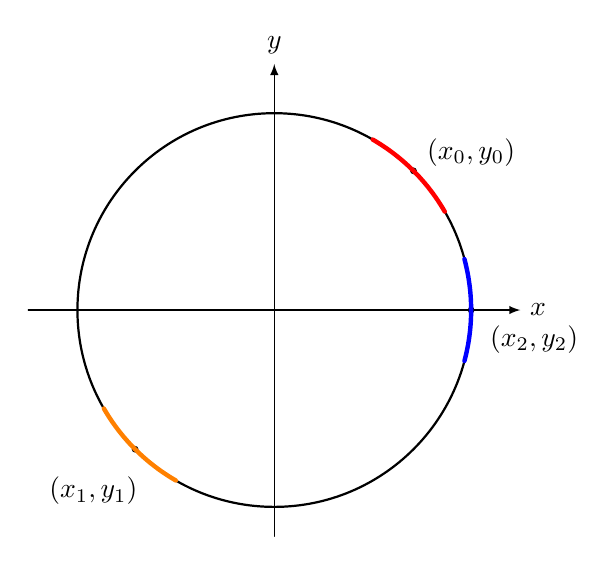
\begin{tikzpicture}[scale=2.5,cap=round,>=latex]
        % draw the coordinates
        \draw[->] (-1.25cm,0cm) -- (1.25cm,0cm) node[right,fill=white] {$x$};
        \draw[->] (0cm,-1.15cm) -- (0cm,1.25cm) node[above,fill=white] {$y$};

        % draw the unit circle
        \draw[thick] (0cm,0cm) circle(1cm);

        \filldraw[black] (45:1cm) circle(0.4pt)
                        (45:-1cm) circle(0.4pt)
                        (0:1cm) circle(0.4pt);

        \draw (1.32cm,-0.15cm) node(b) {$(x_2, y_2)$}
                        (1.0cm,0.8cm) node(a) {$(x_0, y_0)$}
                        (45:-1.3cm) node(c) {$(x_1, y_1)$};
                        
        \draw [red,ultra thick,domain=30:60] plot ({cos(\x)}, {sin(\x)});
        \draw [blue,ultra thick,domain=-15:15] plot ({cos(\x)}, {sin(\x)});
        \draw [orange,ultra thick,domain=210:240] plot ({cos(\x)}, {sin(\x)});
    \end{tikzpicture}
\end{center}
Если мы изобразим решения этого уравнения, то получится единичная окружность.
Зафиксируем на ней точку $(x_0, y_0)$. 
Если мы будем сдвигаться от нее немного влево и вправо, то у нас получится график функции.

Мы даже можем легко понять, как устроена эта функция: $g(x) = \sqrt{1 - x^2}$.
Так вот такая функция называется неявно заданной уравнением $x^2 + y^2 = 1$.

Если же мы зафиксируем точку $(x_1, y_1)$, то неявная функция примет вид $g(x) = -\sqrt{1 - x^2}$. 
А для точки $(x_2, y_2)$ это уже будет $h(y) = \sqrt{1 - y^2}$. 
Заметим, что для двух предыдущих точек мы также могли записать функцию для $y$.

Теорема о неявной функции как раз и говорит о том, в каком случае мы можем написать неявную функцию для конкретной переменной в конкретной точке.
